\documentclass[a4paper]{article}

\usepackage{caption}
\usepackage{listings}
\usepackage{fancyhdr}
\usepackage[top=3cm,bottom=3cm,left=3cm,right=3cm]{geometry}
\usepackage{color}
\usepackage{amsmath}
\usepackage{graphicx}
\usepackage{tabulary}
\usepackage{siunitx}
\usepackage{caption}

\definecolor{dkgreen}{rgb}{0,0.6,0}
\definecolor{gray}{rgb}{0.5,0.5,0.5}
\definecolor{mauve}{rgb}{0.58,0,0.82}

\lstset{frame=tb,
  language=Octave,
  aboveskip=3mm,
  belowskip=3mm,
  showstringspaces=false,
  columns=flexible,
  basicstyle={\small\ttfamily},
  numbers=none,
  numberstyle=\tiny\color{gray},
  keywordstyle=\color{blue},
  commentstyle=\color{dkgreen},
  stringstyle=\color{mauve},
  breaklines=true,
  breakatwhitespace=true,
  tabsize=3
}

\newcommand{\HRule}{\rule{\linewidth}{0.5mm}}
\pagestyle{fancy}
\lfoot{\small \color{gray}Tom Peerdeman - 10266186}
\cfoot{\thepage}
\rfoot{\small \color{gray}Ren\'e Aparicio Sa\'ez - 10214054}
\lhead{\small \color{gray}Autonome Mobiele Robots}

\begin{document}
\begin{titlepage}
\begin{center}
\textsc{\Large Autonome Mobiele Robots}\\[0.5cm]
\HRule \\[0,4cm]
\textsc{\huge \bfseries NXT - Particle filter based simultaneous localization and mapping}
\HRule \\[8cm]
\begin{minipage}{0.4\textwidth}
\begin{flushleft}\large
\emph{Auteurs: Tom Peerdeman \& Ren\'e Aparicio Saez}\\
\end{flushleft}
\end{minipage}
\begin{minipage}{0.4\textwidth}
\begin{flushright}\large
\emph{Datum: \today\\\hspace{1cm}}\\
\end{flushright}
\end{minipage}
\end{center}
\end{titlepage}

\tableofcontents
\newpage

\section{Materiaal}
Om de experimenten uit dit rapport te kunnen uitvoeren zijn de volgende materialen gebruikt:\\
- PC/Laptop met Matlab\\
- Boek: Autonomous Mobile Robots 2th Edition - Roland Siegwart et al.\\
- NXT-Robot\\
- Logitech Webcam\\
- Gloeilamp\\
- Zwarte tape

\section{Introduction}
Een autonome mobiele robots moet een kaart kunnen opbouwen van zijn omgeving. Aan de hand van zijn eigen gemaakte kaart zou hij met behulp van bekende kaarten kunnen bepalen waar hij zich in de wereld bevindt. Een veel gebruikte methode om een kaart al rijdend op te bouwen is SLAM (Simultaneous Localization And Mapping). Er kan dan met een bepaalde zekerheid bepaald worden waar de robot zich momenteel bevindt. Het is de bedoeling dat de robot in een gebied rond kan rijden en hierbij een goede kaart kan maken. Zo moet hij bijvoorbeeld na het rijden van een rondje weer hetzelfde deel van de kaart zien (mits er niks veranderd is aan de omgeving).

\section{Feature detection}
\label{sec:featdetc}
De gebruikte versie van SLAM, fastSLAM, maakt gebruik van ruwe odometrie data en features welke gedetecteerd worden door de laserscan.
Als feature zal gebruik gemaakt worden van hoeken van lijnen. Om de corners te kunnen vinden zullen eerst de lijnen gevonden moeten worden uit de ruwe punten data die de laserscan aanlevert. Om deze lijnen te kunnen detecteren wordt gebruik gemaakt van het split \& merge algoritme. Het split en merge algoritme is in stappen uitgelegd in listing \ref{lst:splitmerge}.

\begin{lstlisting}[caption= Split \& merge algorithm, label=lst:splitmerge, numbers=left]
Initially: set s1 consists of all N points. Insert s1 to the list L. Set index i=1
Fit a line to the next set si in L
Detect the point P with the maximum distance D to the line
if D is less than a threshold then continue to step 2
else split si at P into si1 and si2, replace si , in L, by si1 and si2. Continue to step 2
When all sets (segments) in L have been checked, merge collinear segments.
\end{lstlisting}

\noindent Het fitten van een lijn wordt hierbij gedaan door het zoeken naar een lijn zodanig dat de som van de afstanden in het kwadraat van de punten tot de lijn minimaal is. De lijn wordt hierbij uitgedrukt in polaire co\"ordinaten $r$ en $\alpha$ (zie figuur \ref{fig:linefit}). 
Dit is het geval wanneer de formule $D^2 = \sum\limits_{i=1}^n r-x_i cos(\alpha) - y_i sin(\alpha)$ minimaal is. Om de waardes van $r$ en $\alpha$ te kunnen vinden kan gebruik gemaakt worden van de afgeleiden, $\frac{d(D^2)}{dr} = 0$ en $\frac{d(D^2)}{d\alpha} = 0$.
Hieruit worden de volgende vergelijkingen verkregen:\\
$nom =  -2\sum\limits_{i=1}^n (x_i - x_c)(y_i - y_c)$\\
$dennom =  \sum\limits_{i=1}^n (y_i - y_c)^2 - (x_i - x_c)^2$\\
$\alpha = 0.5\mbox{ atan2}(nom, denom)$\\\\
Hierbij zijn $x_c$ en $y_c$ de co\"ordinaten van het middelpunt van alle punten. Om deze co\"ordinaten te vinden wordt simpelweg het gemiddelde van de $x$ en het gemiddelde van de $y$ waarden van alle punten genomen. Aan de hand van de $\alpha$ parameter kan de $r$ parameter worden gevonden.
Het is namelijk zo dat een punt op een lijn uitgedrukt in polaire co\"ordinaten voldoet aan de vergelijking $x cos(\alpha) + y sin(\alpha) = r$. De $r$ parameter kan worden gevonden als we van een punt zeker weten dat het op de lijn ligt. Dit punt valt niet exact te bepalen, daarom is gekozen om gebruik te maken van de gemiddelde waardes van x en y om daaruit de waarde voor r te verkrijgen. De gemiddelde waardes zullen vrij dicht in de buurt komen van een punt op de lijn.

Als nu naar de punten wordt gekeken die het verste op de lijn liggen kunnen de uiteindes van dit lijnsegment bepalen worden bepaald. Het wordt nu ook makkelijker om hoeken te zoeken door alleen naar deze uiteindes te kijken en te bekijken of ze een hoek vormen met een ander lijnsegment. 

\begin{figure}[h]
	\centering
	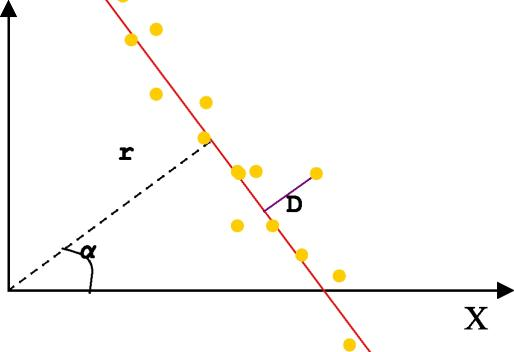
\includegraphics[width=0.7\textwidth]{img/stolenline.png}
	\caption{Fitten van de lijn door de som van D kwadraat te minimaliseren}
	\label{fig:linefit}
\end{figure}

\section{fastSLAM algoritme}
Het fastSLAM algoritme maakt gebruik van particles. Hierbij kan elk particle voorgesteld worden als een kans dat de robot aanwezig is op de positie van de robot, de stand van de robot maakt hierbij ook deel uit van de positie. Het algoritme werkt met twee stappen.\\
Stap 1 is de odometrie update. In deze stap wordt gekeken naar de verplaatsing van de robot. Aan de hand van de encoderwaardes kan worden uitgerekend welke afstand gereden is. Aangezien de kans op een verschil tussen de gemeten waarde en de echt afgelegde afstand groeit kan worden voorspeld dat de particles zich met een bepaalde error zullen voortbewegen. Er wordt aangenomen dat deze error gaussisch is. De nieuwe positie van een particle kan dan worden voorspeld met de vergelijking \\\\
$
\begin{bmatrix}
x\\
y\\
\theta
\end{bmatrix}^{t+1}
=
\begin{bmatrix}
(x_t + dr_n cos(dth_n + \theta_t))\\
(y_t + dr_n sin(dth_n + \theta_t)) \\
pi2pi(pi2pi(\theta) + dth)
\end{bmatrix}
$\\\\
Hierbij is $pi2pi$ een functie die hoeken omzet van de range $[0 2\pi]$ naar $[0,pi], (-pi, 0]$.
$dth_n$ is de toegevoegde noise voor de afgelegde hoek $dth$.
$dr_n$ is de toegevoegde noise voor de afgelegde afstand.\\
Het is belangrijk te vermelden dat er meerdere odometrie updates kunnen voorkomen voordat stap 2 uitgevoerd wordt. Hierdoor kan de error in de particle positie vrij hoog oplopen. Deze error moet dat naar beneden gebracht worden door de data uit de laserscan (stap 2).\\
\\
Stap 2 is de laserscan update. In de laserscan update wordt de error verkleind door een aantal particles weg te gooien. De particles die worden weggegooit hebben daarbij de kleinste kans dat de robot op de positie van deze particles is. Dit wordt gedaan door de ruwe laserscan data om te zetten in features (hoeken in dit geval) zoals is uitgewerkt in sectie \ref{sec:featdetc}. Als de gedetecteerde features al eens eerder gedetecteerd waren kunnen een aantal particles worden weggegooit aangezien de positie van deze features al bekend is. Door voor elk particle te voorspellen waar de feature zich zou moeten bevinden als de robot op die positie zou zijn, en dit te vergelijken met de gedetecteerde positie kan elke particle een gewicht krijgen. Dit gewicht is hoger naar mate de gedetecteerde positie meer overeenkomt met de voorspelde positie. Aan de hand van deze weights gaat het algoritme de particle set resamplen. De particles met de laagste weights worden hierbij verwijderd. Aangezien de overgebleven particles weer een error met een bepaalde distributie voorstellen kunnen uit deze distibutie nieuwe posities worden getrokken om zo het aantal particles gelijk te houden aan het aantal van voor de resampling.

\section{Schatten van SLAM parameters}
SLAM maakt gebruik van enkele parameters. Deze parameters moeten worden geschat, om het beste resultaat te verkrijgen. Met behulp van een meegeleverde test log, kunnen enkele experimenten met verschillende waarden voor deze parameters worden gedaan. De te schatten parameters zijn, $NPARTICLES$, $sigmaX$, $sigmaTH$, $sigmaR$ en $sigmaB$. $NPARTICLES$ geeft aan hoeveel deeltjes (locaties) er moeten worden weergegeven waar de robot momenteel kan zijn. $sigmaX$ en $sigmaTH$ geven de variantie in de odometrie aan, de afwijking van de gegeven waarden voor respectievelijk de gereden afstand en de hoek. $sigmaR$ en $sigmaB$ geven de variantie aan die de laserscan als afstanden tot lijnen teruggeeft (de rangesensor).
\subsection{Experimenten}
In figuur \ref{fig:npart}, figuur \ref{fig:odoexp} en figuur \ref{fig:rangeexp}\footnote{deze figuren staan aan het einde van dit labreport, i.v.m. structuur behoudt van het labreport} zijn de resultaten te zien van de gemaakt experimenten. Duidelijk is te zien dat met het verhogen van het aantal $NPARTICLES$ de dikte van de lijn gestaag toeneemt. Door $NPARTICLES =200$ te kiezen wordt ervoor gezorgd dat de lijn niet te dun wordt en niet te dik.\\
Zoals te verwachten viel, is met een lage variantie in de odometrie minder ruis voor de gedetecteerde muren zichtbaar. Deze variantie moet dus laag gehouden worden om nog een duidelijke kaart te kunnen opbouwen. Een variantie van $sigmaX=0.00003m$ en $sigmaTH=\SI{0.0002}{\degree}$ zorgt voor een duidelijk resultaat.\\
Opvallend is het extreem dikker worden van de locatie van de robot zodra een lage variantie wordt gekozen voor de rangesensor. De rangesensor is blijkbaar niet gevoelig genoeg om met grote zekerheid de werkelijke afstand terug te geven, dus moet een grotere waarde voor de variantie worden gekozen. $sigmaR=0.7$ en $sigmaB=0.7$ levert een niet al te dikke locatielijn op, en een duidelijk resultaat voor de locatie van de muren.

\section{Deel 2, Eigen data}
\subsection{Offline SLAM met behulp van een dataset}
Er moet worden gewerkt met een offline dataset, in verband met tijdgebrek en het niet aanwezig zijn van voldoende robots. De meegeleverde dataset bestaat uit 61 fotos.
Voordat begonnen kan worden met het opbouwen van een kaart moeten eerst de parameters voor de camera worden gecalibreerd. De fotos bevatten echter twee verschillende centers. Na het 40e plaatje veranderd de center enigszins (Picture 51.jpg tot het einde van de dataset). De centers zijn respectievelijk $centre_1 = [465;343]$ voor de eerste 40 fotos en $centre_2=[465;335]$ voor de overige fotos. Alle fotos maken gebruik van $\alpha = 140$ en $Rmin = 100$ en $Rmax = 180$. Er is gebruik gemaakt van een BWtreshold van 100, behalve voor Picture 17.jpg tot Picture 22.jpg. Hierbij is de treshold verlaagd naar 90. Dit is gedaan omdat bij deze fotos de draad die de camera met de laptop verbind gemeten wordt. De draad beinvloed hiermee de data. In figuur \ref{fig:route} is te zien welke route gereden is.
Deze kaart met bijbehorende route zal ongeveer overeen moeten komen met de opgebouwde kaart door het SLAM algoritme.
\begin{figure}[h]
	\centering
	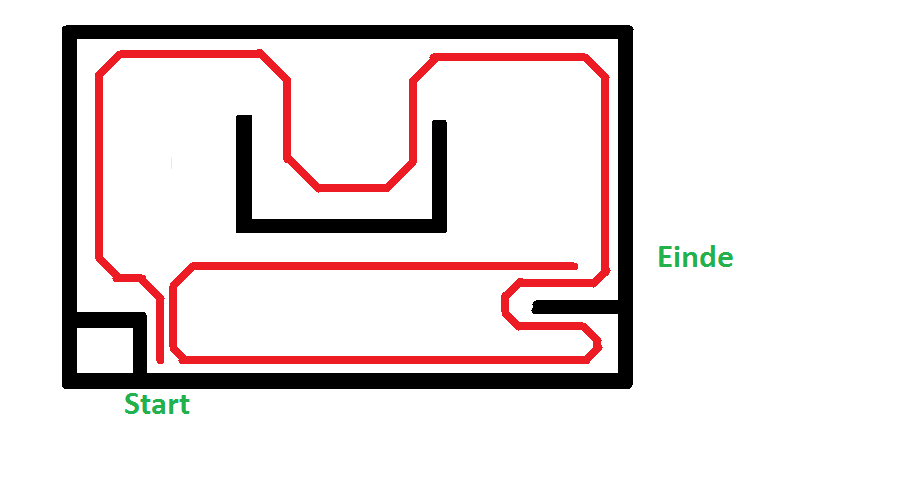
\includegraphics[width=0.8\textwidth]{matlab/imgs/route.png}
	\caption{Afgelegde route}
	\label{fig:route}
\end{figure}

\subsection{Odometrie bepalen}
Omdat er gebruik gemaakt wordt van een dataset van fotos en niet van de meegeleverde GUI, moet de odometrie met de hand worden gemaakt. Aan de hand van de meegegeven layout, te zien in figuur \ref{fig:layout}, en het bekijken van de locatie van de robot aan de hand van de fotos kan een schatting gemaakt worden van de afgelegde afstanden.
\begin{figure}[h]
	\centering
	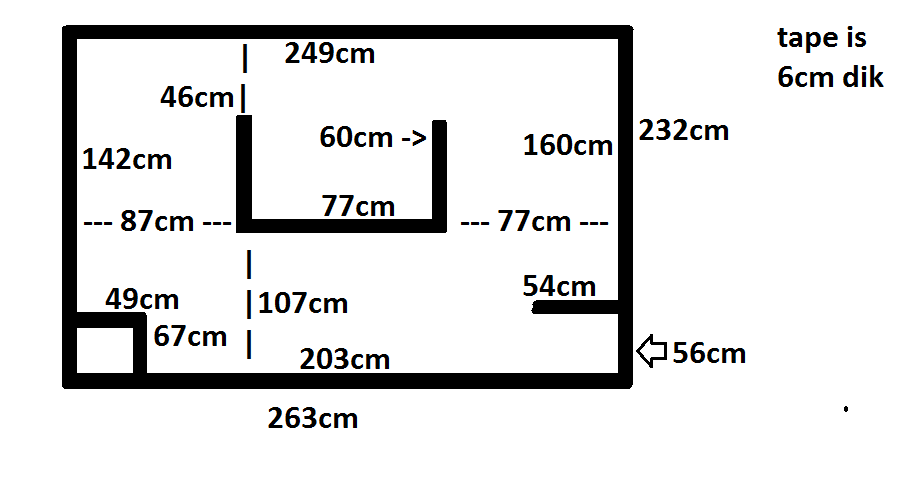
\includegraphics[width=0.8\textwidth]{matlab/imgs/layout.png}
	\caption{Layout van de kaart}
	\label{fig:layout}
\end{figure}
Deze schatting kan aan de hand van experimenten worden geoptimaliseerd. Deze optimalisatie wordt gedaan door afgelegde afstanden te vergroten of te verkleinen. In een enkel geval moet de draaihoek worden aangepast. De meeste bochten die gemaakt worden bestaan uit twee korte bochten van elk $\SI{45}{\degree}$. Er zijn echter twee bochten waarbij eerst een draaiing wordt gemaakt van $\SI{60}{\degree}$ gevolgd door een draaiing van $\SI{30}{\degree}$.
\subsection{Resultaten}
Het resultaat met geoptimaliseerde odometrie is zichtbaar in figuur \ref{fig:final}. Er is duidelijk zichtbaar dat de gevonden kaart grotendeels overeenkomt met de layout uit figuur \ref{fig:route}. De gemaakte kaart is een kwartslag gedraaid, maar dit maakt voor de metingen niet uit. De gevonden afstanden voor de lengtes van de lijnen klopt in grote lijnen. 
\begin{figure}[h]
	\centering
	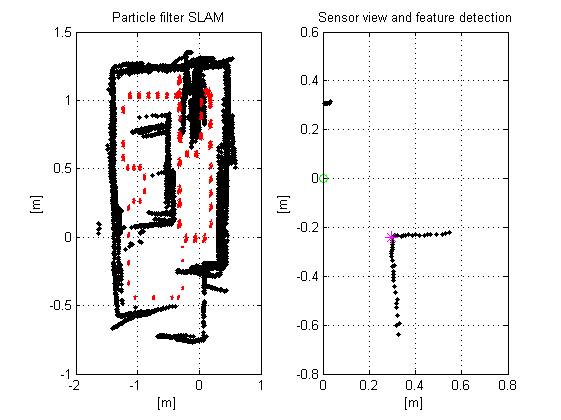
\includegraphics[width=0.7\textwidth]{img/statusnow.png}
	\caption{Uiteindelijk resultaat}
	\label{fig:final}
\end{figure}
\subsection{Discussie}
Er is ruis zichtbaar in het resultaat. Dit heeft te maken met het mogelijk nog meer te optimaliseren van de odometrie of door het optimaliseren van de parameters.
Omdat de dataset twee verschillende centers heeft, ontstaat ruis vanaf plaatje 41. Dit zorgt voor meer ruis (de dikkere muur) rechtsboven in figuur \ref{fig:final}.\\
De gevonden afstanden kloppen grotendeels. Ze zijn niet volledig accuraat vanwege meerdere factoren. Zo speelt de ruis een grote rol, maar ook de omzetting van het gebolde beeld naar een 2D-beeld zorgt voor een significante afwijking. Omdat de bolling van de gebruikte gloeilamp niet een perfecte bolling is, is het moeiilijk om een goede alpha te kiezen waarbij de werkelijke afstand klopt ten opzichte van de pixelwaarden, zonder dat het beeld vervormd raakt. Dit zorgt voor een kleine afwijking in werkelijke afstanden.
\subsection{Verbeteringen}
De odometrie houdt momenteel alleen rekening met de afgelegde afstand in de huidige rijrichting van de robot. Het is hierdoor niet mogelijk om met behulp van fotos een daadwerkelijke bocht aan te geven. Het algoritme denkt nu dat er een rechte lijn wordt gereden en vervolgens wordt gedraaid, in plaats van een continue draaiing over de af te leggen afstand uit te voeren. Daarnaast zullen er betere resultaten worden verkregen als er per locatie meerdere metingen worden gemaakt en de afstand tussen de metingen verkleind wordt. Daar komt bij dat tijdens het maken van de dataset het aan te raden is de afgelegde afstanden en draaihoeken worden opgeschreven, zodat deze niet achteraf geschat hoeven te worden. Tot slot zou een verbeterde omni-directionele camera, die op een juiste manier de pixelafstanden om kan zetten naar werkelijke afstanden een uitkomst bieden op betere resultaten.
\newpage
\section{Parameter experimenten figuren}
\begin{figure}[h]
\captionsetup{justification=centering}
\begin{center}$
\begin{array}{cc}
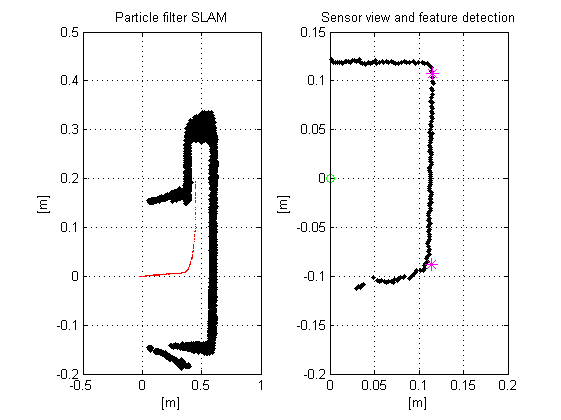
\includegraphics[width=0.5\textwidth]{{img/slam5particles}.png} &
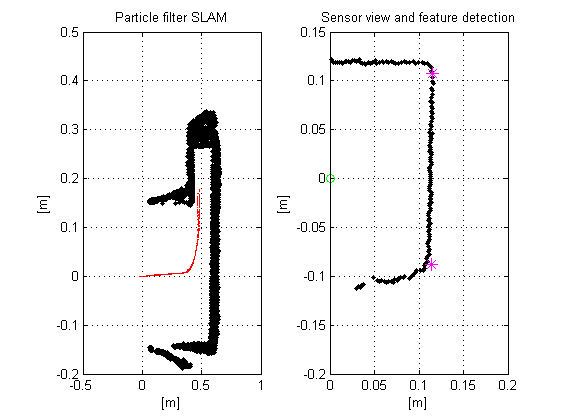
\includegraphics[width=0.5\textwidth]{{img/slam20particles}.png}\\
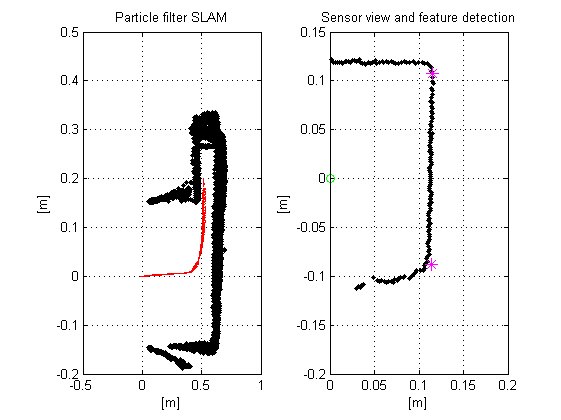
\includegraphics[width=0.45\textwidth]{{img/slam100particles}.png} &
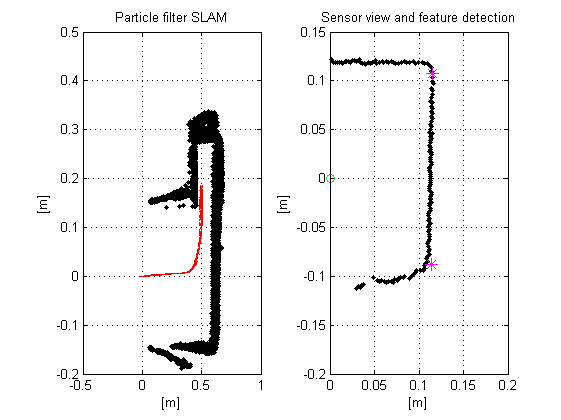
\includegraphics[width=0.45\textwidth]{{img/slam200particles}.png}
\end{array}$
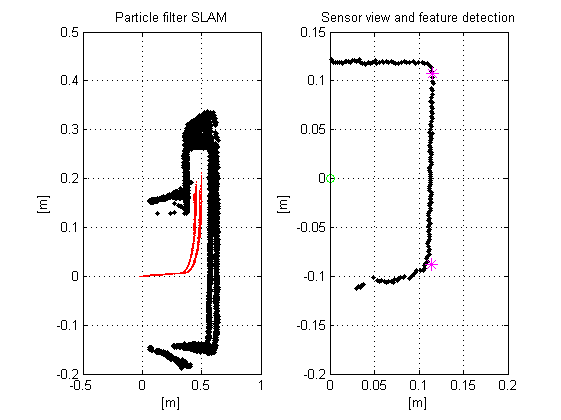
\includegraphics[width=0.45\textwidth]{{img/slam1000particles}.png}
\end{center}
\caption{Het aantal $NPARTICLES$,\\linksboven $NPARTICLES=5$, rechtsboven $NPARTICLES=20$\\linksmidden $NPARTICLES=100$, rechtsmidden $NPARTICLES=200$\\Onderaan $NPARTICLES=1000$}
\label{fig:npart}
\end{figure}

\begin{figure}[h]
\captionsetup{justification=centering}
\begin{center}$
\begin{array}{cc}
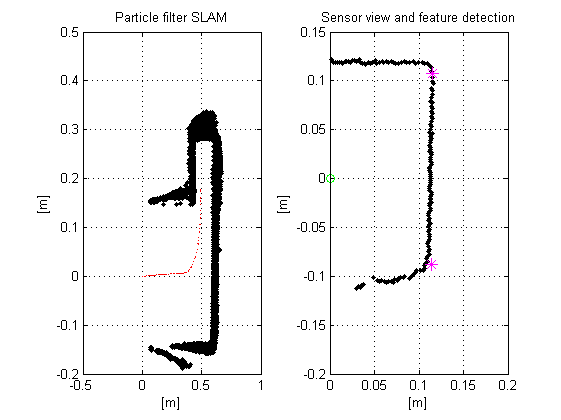
\includegraphics[width=0.5\textwidth]{{img/slam0.00003-0.0002odonoise}.png} &
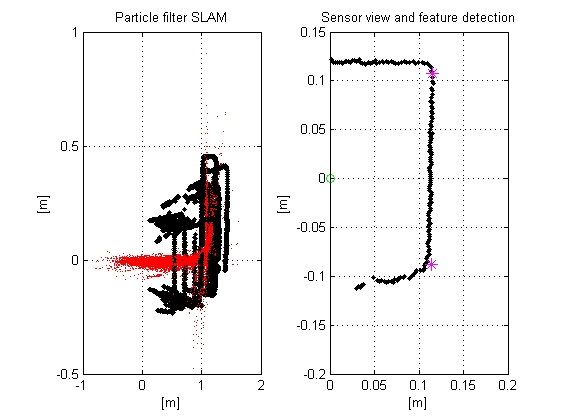
\includegraphics[width=0.5\textwidth]{{img/slam0.3-0.2odonoise}.png}
\end{array}$
\end{center}
\caption{Odometrie variantie,\\ links $sigmaX=0.00003m$ en $sigmaTH=\SI{0.0002}{\degree}$ \\ rechts $sigmaX=0.3m$ en $sigmaTH=\SI{0.2}{\degree}$}
\label{fig:odoexp}
\end{figure}

\begin{figure}[h]
\captionsetup{justification=centering}
\begin{center}$
\begin{array}{cc}
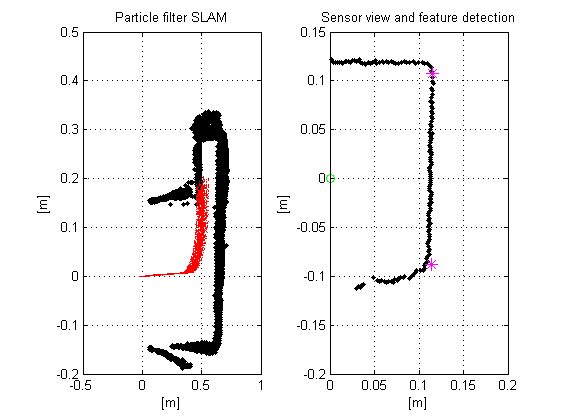
\includegraphics[width=0.5\textwidth]{{img/slam0.0001-0.0001lasernoise}.png} &
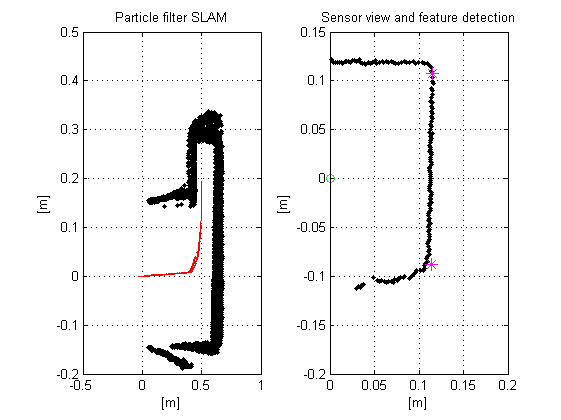
\includegraphics[width=0.5\textwidth]{{img/slam0.7-0.7lasernoise}.png}
\end{array}$
\end{center}
\caption{Rangesensor variantie,\\ links $sigmaR=0.0001$ en $sigmaB=0.0001$ \\ rechts $sigmaR=0.7$ en $sigmaB=0.7$}
\label{fig:rangeexp}
\end{figure}
\clearpage
\section{Code snippets}
Hieronder zijn enkele code snippets te vinden van files die flink zijn aangepast ten opzichte van hoe ze zijn geleverd.\\
FitLine.m bevat de code om de hoek en de afstand tot een lijn te bepalen.
\begin{lstlisting}[caption= Fitline.m, label=lst:checkconcat, numbers=left]
%---------------------------------------------------------------------
% This function computes the parameters (r, alpha) of a line passing
% through input points that minimize the total-least-square error.
%
% Input:   XY - [2,N] : Input points
%          
% Output:  r, alpha: paramters of the fitted line

function [r, alpha] = FitLine(XY)
  
  % Compute the centroid of the point set (xmw, ymw) considering that 
  % the centroid of a finite set of points can be computed as
  % the arithmetic mean of each coordinate of the points.

  % XY(1,:) contains x position of the points
  % XY(2,:) contains y position of the points  

  xmw = mean(XY(1,:));
  ymw = mean(XY(2,:));

  % compute parameter alpha (see exercise pages)
  nom = 0;
  denom = 0;
  for i=1:size(XY,2)
      nom = nom + ((XY(1,i) - xmw) * (XY(2,i) - ymw));
      denom = denom + ((XY(2,i) - ymw)^2 - (XY(1,i) - xmw)^2);
  end
  
  nom = -2 * nom;
  
  alpha = 0.5 * atan2(nom, denom);
  
  % compute parameter r (see exercise pages)
  r = xmw * cos(alpha) + ymw * sin(alpha);
  
  % Eliminate negative radii
  if r < 0,
    alpha = alpha + pi;
    if alpha > pi, alpha = alpha - 2 * pi; end
    r = -r;
  end;
  
  return  % function FitLine
\end{lstlisting}
\newpage
\noindent
predict\_odo.m bevat de code die de odometrie voorspelt aan de hand van meegegeven variantie parameters.
\begin{lstlisting}[caption= predict\_odo.m, label=lst:checkconcat, numbers=left]
function particle = predict_odo(particle, dr, dth, Q)
% Q  cov matrix, noise odometry
% dr and dth is retrieved from the encoders (that is delta_r and delta_theta) in dt
% time.

Dmv = multivariate_gauss([dr; dth], Q, 1);
dr_n = Dmv(1); 
dth_n = Dmv(2);


% predict state
xv= particle.xv;

% xv contains the *LAST* position of the considered particle in world coordinate frame, such as:
% xv(1) = last x
% xv(2) = last y
% xv(3) = last theta

% In order to obtain the prediction step for the current particle 'particle'
% consider then the measurements of the odometry of the robot that are:
% dr_n  = noise added measurement of dr using  cov. matrix Q
% dth_n = noise added measurement of d_th using  cov. matrix Q

% Hint:
% x_new = x_old + dn_rn*cos(dth_rn + theta_old)

particle.xv= [ (xv(1) + dr_n * cos(dth_n + xv(3))) ; 
               (xv(2) + dr_n * sin(dth_n + xv(3))) ;
              pi_to_pi(pi_to_pi(xv(3)) + dth)];
 
 
% pi_to_pi is a *safe* function that converts angles from [0,2*pi] into the
% standard convention {[0,pi], (-pi, 0]}
\end{lstlisting}
logger/MainOffline.m bevat de code voor het opbouwen van de log voor de gebruikte offline dataset.
\begin{lstlisting}[caption= logger/MainOffline.m, label=lst:checkconcat, numbers=left]
% =================================================================
% 
%  Main.m
%  Closed-loop position control for differential-drive robots.
% 
%  The calling syntax is:
%       Main
%
%  Reference:
%  Introduction to: Autonomous Mobile Robots, Chapter 3.
% 
%  This is an M-file for MATLAB.  
%  Tested in: Matlab 7.1.0
%  Date: 12.04.07
%
% =================================================================*/

clc; % clear console

path(path, './scans/');
path(path, './odometry/');

load('est_odo.mat');


%===================================%
%   PARAMETERS TO CHANGE            %
%===================================%

% NUMBER OF SCANS:
N = 360;

% TIME BETWEEN TWO SNAPSHOTS:
T_b_S = 0.5;  %[s]

% FREQUENCY OF ODOMETRY UPDATE:
F_O_U = 5;  %[Hz]

% NAME OF THE LOG FILE:
Log_name = 'log.txt';

%===================================%

% Open the log file for writing the data
FILE = fopen(Log_name, 'w')

tic;
for i=1:61
    % Schat hier dx en dtheta
    dx = est_odo(i, 1);
    dtheta = deg2rad(est_odo(i, 2));
    SaveEncoderData(FILE, toc, dx, dtheta, N);

    disp(sprintf('Taking laser data %d', (i + 10)));
    laser_scans = GetLaserScans(N, i+10);
    SaveLaserData(FILE, toc, laser_scans); 
    
    pause(T_b_S);
end

fclose(FILE);

display('Execution Complete!');
\end{lstlisting}

\end{document}
